\documentclass[11pt]{article}

% Basic setup
\usepackage{cmap}
\usepackage[utf8]{inputenc}
\usepackage[T2A]{fontenc}
\usepackage[english]{babel}

% Sans serif font by default
\renewcommand\familydefault{\sfdefault}

% Document margins
\usepackage[margin=2.5cm]{geometry}

% \includegraphics, used to include a picture of me
\usepackage{graphicx}

% === Typography ===

% == Boxes ==
\usepackage{adjustbox}
\usepackage{calc}
\usepackage{tabularx}

% == Colors ==
\usepackage[usenames,dvipsnames]{color}
\definecolor{CvRuleColor}{gray}{0.5}
\definecolor{CvWorkplaceHeaderColor}{gray}{0.97}

% == URLs ==
\usepackage[colorlinks=true,urlcolor=blue]{hyperref}

% == Paragraphs ==
\usepackage{parskip}
\setlength\parindent{0cm}
\setlength\parskip{0cm}

% == Lists ==
\usepackage{enumitem} % [noitemsep]

% === Custom commands ===

% "C++", thanks to this guy: http://tex.stackexchange.com/a/4304/9088
\usepackage{relsize}
\newcommand\CXX{C\nolinebreak[4]\hspace{-.05em}\raisebox{.4ex}{\relsize{-3}{\textbf{++}}}}

% Whitespace
\newcommand\CvSmallSkipLength{0.5em}
\newcommand\CvBigSkipLength{1em}

\newcommand\CvSkip[1]{\vspace{#1}}

\newcommand\CvSmallSkip{\CvSkip{\CvSmallSkipLength}}
\newcommand\CvBigSkip{\CvSkip{\CvBigSkipLength}}

% Section headers ("Experience", "Education", etc.)
\newcommand\CvSectionHeader[1]{\CvBigSkip\textbf{#1}\CvBigSkip}

% Horizontal line/separator
\newcommand\CvRule{\begingroup\color{CvRuleColor}\hrule\endgroup}

% Workplace header
\newcommand\CvWorkplaceHeader[5]{\begingroup%
  \CvRule%
  \fboxsep0pt%
  \colorbox{CvWorkplaceHeaderColor}{%
    \begin{minipage}{\linewidth-2\fboxsep}%
\CvSmallSkip%
#1 -- #2 \hfill \textit{#3} at #4 (\href{http://#5/}{#5})%
\CvSmallSkip%
    \end{minipage}%
  }%
  \CvRule%
\endgroup%
}

% Workplace description
\newenvironment{CvWorkplaceDescription}{%
    \begingroup\setlength\parskip{\CvSmallSkipLength}%
  }{%
    \CvSmallSkip\endgroup%
  }

\pagestyle{empty}

\begin{document}

\adjustbox{valign=t}{%
  \begin{minipage}{3.5cm}%
    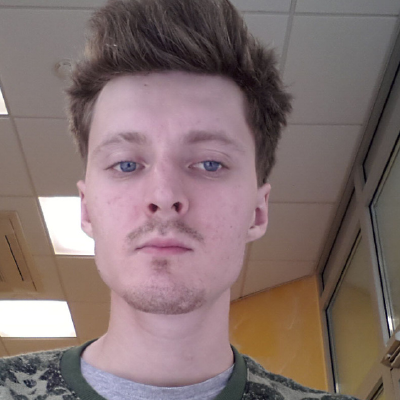
\includegraphics[width=3.5cm]{img/selfie_face.png}
  \end{minipage}%
}%
\hfill%
\adjustbox{valign=t}{%
  \begin{minipage}{\linewidth-3.5cm-\CvBigSkipLength}%
{\bfseries\large Alexey Polusov}\\*
{\color{CvRuleColor} Last updated on: \today}
    \CvBigSkip
    \CvRule
    \CvSmallSkip
    \begin{tabularx}{\textwidth}{@{}lX}
email: & \href{mailto:lectricas@gmail.com}{lectricas@gmail.com} \\
github: & \href{https://github.com/lectricas/}{https://github.com/lectricas/} \\
tel.: & +7\,(952)\,377-09-69 \\
Address: & 1 Tatarskiy Pereulok, apt. 7 \\
& Saint Petersburg, Russia, 197198 \\
    \end{tabularx}%
    \CvSmallSkip
    \CvRule
  \end{minipage}%
}

\CvSectionHeader{Experience}

\CvWorkplaceHeader{October 2018}{Current time}{Android developer}{Firstline Software}{firstlinesoftware.com}
\begin{CvWorkplaceDescription}
Solo development of mid-scale apps
\begin{itemize}[noitemsep]
  \item developed a medical app from scratch
 \item  app's key feature is a custom view consist of a infinite graph with scaling and Bezier curve. 
  \item spend a month on the research, finally found an elegant solution for the graph
  \item took another project for refactoring and feature implementing
  \item trying get a second android dev project team in order to teach him
  \item done a small talk about presentation patterns and why it matters to my colleges, made local Android chat
\end{itemize}

Key skills \& technologies employed:
\begin{itemize}[noitemsep]
  \item Kotlin, Koin, RxPM, Room, RxBindings, RxJava, Retrofit
  \item conversations, negotiations
\end{itemize}
\end{CvWorkplaceDescription}

\CvWorkplaceHeader{September 2017}{October 2018}{Android developer}{MobileUp}{mobileup.ru}

\begin{CvWorkplaceDescription}
I have been taking part in development of several projects, from mid-scale to large ones:
\begin{itemize}[noitemsep]
  \item participated in developing a blockchain-oriented application(+ etherium currency involved),
  \item responsible for all UI logic, I've done tons of compound views and native animations(the app is for entertainment and it is beautiful)
  \item get acquainted with blockchain development
  \item fixed a few other projects adding some cool new features,
  \item configured Bitbucket CI was trying others: Jenkins, AppCenter(we lack some devices), TeamCity,
\end{itemize}

Key skills \& technologies employed:
\begin{itemize}[noitemsep]
  \item Kotlin for sure!,
  \item RxPm(MVVM like library baked in MobileUp),
  \item RxJava, Dagger2, Koin, RxBinding, Conductor, web3j for blockchain
  \item tried Room, Architecture Components, BiometricPrompt, etc
\end{itemize}
\end{CvWorkplaceDescription}

\CvWorkplaceHeader{February 2016}{August 2017}{Android developer}{65apps}{www.65apps.com}

\begin{CvWorkplaceDescription}
I have been taking part in development of a mid-scale projects as a member of an Android team. I was responsible for developing different app features and support components:
\begin{itemize}[noitemsep]
  \item done one middle-size news project from scratch(GP published and successful),
  \item developed multiply features for several projects,
  \item bug fixes for projects on "support",
\end{itemize}

Key skills \& technologies employed:
\begin{itemize}[noitemsep]
  \item Java programming in Android Studio,
  \item CLEAN architecture supported by Dagger 2 and Moxy,
  \item RxJava, Retrofit, Firebase, Butterknife, etc
  \item GitFlow
\end{itemize}
\end{CvWorkplaceDescription}

\CvWorkplaceHeader{June 2015}{December 2015}{Android developer}{Astarus}{astatus.ru}

\begin{CvWorkplaceDescription}
I maintained and extended a mid-scale geo-based project that was already in production.
This Service was used to calculate fuel consumption of the trucks.

Key skills \& technologies employed:
\begin{itemize}[noitemsep]
  \item Java programming in Android Studio,
  \item Google location Api, AsyncTask, etc.
\end{itemize}
\end{CvWorkplaceDescription}

\CvWorkplaceHeader{August 2013}{March 2014}{Software Engineer}{Mark - itt}{mark.ru}

\begin{CvWorkplaceDescription}
I was working in a team of networking experts/software engineers in a Internet Service Provider in Izhevsk city. My daily routing was to make build software tools for technical support team.

Key skills \& technologies employed or studied:
\begin{itemize}[noitemsep]
  \item Perl and Python development,
  \item Oracle and MySQL database manipulation,
  \item parsing data from different model of industrial routers,
  \item Python programming
\end{itemize}
\end{CvWorkplaceDescription}
\CvRule

\CvSectionHeader{Education}

\CvWorkplaceHeader{2009}{2013}{Bachelor of Information Security}{ISTU}{http://istu.ru/}

\begin{CvWorkplaceDescription}
During my education, I've been focusing on the following topics:
\begin{itemize}[noitemsep]
  \item hidden electronic devices for listen in,
  \item hardware key interceptor, masked as a USB - PS/2 adapter
  \item no, I'm not a spy
\end{itemize}
\end{CvWorkplaceDescription}
\CvRule

\begin{minipage}[t]{.5\linewidth}
  \CvSectionHeader{Programming Languages}

  \begin{itemize}
    \item Java, Kotlin, Python
  \end{itemize}

  \CvSectionHeader{Development Tools \& Technologies}

  \begin{itemize}
    \item Bitbucket CI, AppCenter, TeamCity
    \item Heroku, PythonAnywhere, Parse
    \item Git
   \item Bash
  \end{itemize}

  \CvSectionHeader{Hobbies}

  \begin{itemize}
    \item Listening and making music, learning how synthesis works, trying to make my own sounds
    \item math, history of modern Russia, psychology
   \item road bike riding, skiing
  \end{itemize}
\end{minipage}
\begin{minipage}[t]{.5\linewidth}
  \CvSectionHeader{Languages}

  \begin{itemize}
    \item Russian --- mother tongue.
    \item English --- TOEFL 93 score a few years ago(trying to sustain the level).
  \end{itemize}

  \CvSectionHeader{Other Tools \& Technologies}

  \begin{itemize}
    \item postman
   \item Word, Excel, Photoshop
    \item Thinkpad lover, Google Pixel fan
    \item \LaTeX
  \end{itemize}
\end{minipage}

\end{document}